\documentclass[twoside]{book}

% Packages required by doxygen
\usepackage{calc}
\usepackage{doxygen}
\usepackage{graphicx}
\usepackage[utf8]{inputenc}
\usepackage{makeidx}
\usepackage{multicol}
\usepackage{multirow}
\usepackage{textcomp}
\usepackage[table]{xcolor}

% NLS support packages
\usepackage[T2A]{fontenc}
\usepackage[russian]{babel}

% Font selection
\usepackage[T1]{fontenc}
\usepackage{mathptmx}
\usepackage[scaled=.90]{helvet}
\usepackage{courier}
\usepackage{amssymb}
\usepackage{sectsty}
\renewcommand{\familydefault}{\sfdefault}
\allsectionsfont{%
  \fontseries{bc}\selectfont%
  \color{darkgray}%
}
\renewcommand{\DoxyLabelFont}{%
  \fontseries{bc}\selectfont%
  \color{darkgray}%
}

% Page & text layout
\usepackage{geometry}
\geometry{%
  a4paper,%
  top=2.5cm,%
  bottom=2.5cm,%
  left=2.5cm,%
  right=2.5cm%
}
\tolerance=750
\hfuzz=15pt
\hbadness=750
\setlength{\emergencystretch}{15pt}
\setlength{\parindent}{0cm}
\setlength{\parskip}{0.2cm}
\makeatletter
\renewcommand{\paragraph}{%
  \@startsection{paragraph}{4}{0ex}{-1.0ex}{1.0ex}{%
    \normalfont\normalsize\bfseries\SS@parafont%
  }%
}
\renewcommand{\subparagraph}{%
  \@startsection{subparagraph}{5}{0ex}{-1.0ex}{1.0ex}{%
    \normalfont\normalsize\bfseries\SS@subparafont%
  }%
}
\makeatother

% Headers & footers
\usepackage{fancyhdr}
\pagestyle{fancyplain}
\fancyhead[LE]{\fancyplain{}{\bfseries\thepage}}
\fancyhead[CE]{\fancyplain{}{}}
\fancyhead[RE]{\fancyplain{}{\bfseries\leftmark}}
\fancyhead[LO]{\fancyplain{}{\bfseries\rightmark}}
\fancyhead[CO]{\fancyplain{}{}}
\fancyhead[RO]{\fancyplain{}{\bfseries\thepage}}
\fancyfoot[LE]{\fancyplain{}{}}
\fancyfoot[CE]{\fancyplain{}{}}
\fancyfoot[RE]{\fancyplain{}{\bfseries\scriptsize Документация по ip\-\_\-filter. Последние изменения\-: Пт 6 Апр 2018 12\-:42\-:59. Создано системой Doxygen }}
\fancyfoot[LO]{\fancyplain{}{\bfseries\scriptsize Документация по ip\-\_\-filter. Последние изменения\-: Пт 6 Апр 2018 12\-:42\-:59. Создано системой Doxygen }}
\fancyfoot[CO]{\fancyplain{}{}}
\fancyfoot[RO]{\fancyplain{}{}}
\renewcommand{\footrulewidth}{0.4pt}
\renewcommand{\chaptermark}[1]{%
  \markboth{#1}{}%
}
\renewcommand{\sectionmark}[1]{%
  \markright{\thesection\ #1}%
}

% Indices & bibliography
\usepackage{natbib}
\usepackage[titles]{tocloft}
\setcounter{tocdepth}{3}
\setcounter{secnumdepth}{5}
\makeindex

% Hyperlinks (required, but should be loaded last)
\usepackage{ifpdf}
\ifpdf
  \usepackage[pdftex,pagebackref=true]{hyperref}
\else
  \usepackage[ps2pdf,pagebackref=true]{hyperref}
\fi
\hypersetup{%
  colorlinks=true,%
  linkcolor=blue,%
  citecolor=blue,%
  unicode%
}

% Custom commands
\newcommand{\clearemptydoublepage}{%
  \newpage{\pagestyle{empty}\cleardoublepage}%
}


%===== C O N T E N T S =====

\begin{document}

% Titlepage & ToC
\hypersetup{pageanchor=false}
\pagenumbering{roman}
\begin{titlepage}
\vspace*{7cm}
\begin{center}%
{\Large ip\-\_\-filter }\\
\vspace*{1cm}
{\large Создано системой Doxygen 1.8.6}\\
\vspace*{0.5cm}
{\small Пт 6 Апр 2018 12:42:59}\\
\end{center}
\end{titlepage}
\clearemptydoublepage
\tableofcontents
\clearemptydoublepage
\pagenumbering{arabic}
\hypersetup{pageanchor=true}

%--- Begin generated contents ---
\chapter{Список файлов}
\section{Файлы}
Полный список файлов.\begin{DoxyCompactList}
\item\contentsline{section}{\hyperlink{ip__filter_8cpp}{ip\-\_\-filter.\-cpp} }{\pageref{ip__filter_8cpp}}{}
\item\contentsline{section}{\hyperlink{ip__filter_8h}{ip\-\_\-filter.\-h} }{\pageref{ip__filter_8h}}{}
\item\contentsline{section}{\hyperlink{main_8cpp}{main.\-cpp} }{\pageref{main_8cpp}}{}
\item\contentsline{section}{\hyperlink{test__main_8cpp}{test\-\_\-main.\-cpp} }{\pageref{test__main_8cpp}}{}
\item\contentsline{section}{\hyperlink{version_8h}{version.\-h} }{\pageref{version_8h}}{}
\end{DoxyCompactList}

\chapter{Файлы}
\hypertarget{ip__filter_8cpp}{\section{Файл ip\-\_\-filter.\-cpp}
\label{ip__filter_8cpp}\index{ip\-\_\-filter.\-cpp@{ip\-\_\-filter.\-cpp}}
}
{\ttfamily \#include $<$cassert$>$}\\*
{\ttfamily \#include $<$cstdlib$>$}\\*
{\ttfamily \#include $<$iostream$>$}\\*
{\ttfamily \#include $<$string$>$}\\*
{\ttfamily \#include $<$vector$>$}\\*
{\ttfamily \#include $<$algorithm$>$}\\*
{\ttfamily \#include \char`\"{}version.\-h\char`\"{}}\\*
{\ttfamily \#include \char`\"{}ip\-\_\-filter.\-h\char`\"{}}\\*
Граф включаемых заголовочных файлов для ip\-\_\-filter.\-cpp\-:
\nopagebreak
\begin{figure}[H]
\begin{center}
\leavevmode
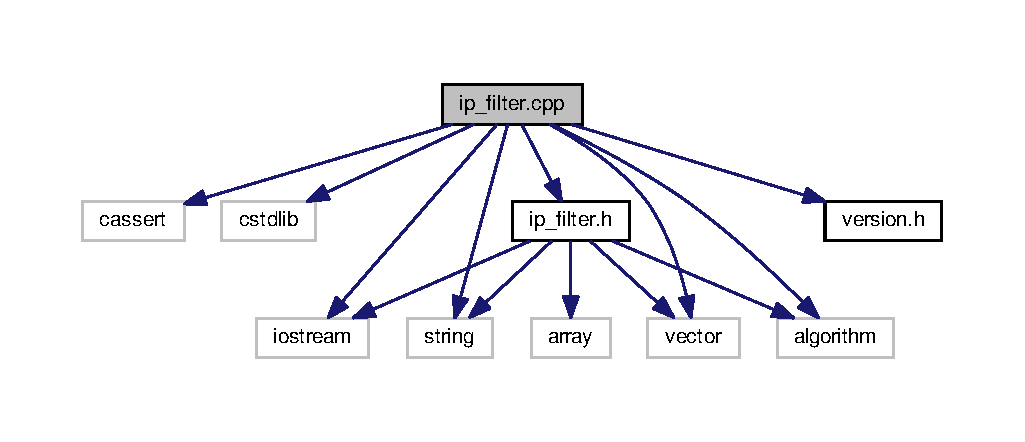
\includegraphics[width=350pt]{ip__filter_8cpp__incl}
\end{center}
\end{figure}
\subsection*{Функции}
\begin{DoxyCompactItemize}
\item 
std\-::vector$<$ std\-::string $>$ \hyperlink{ip__filter_8cpp_a5d67634c85a0d90fa46ad22c5740915c}{split} (const std\-::string \&str, char d)
\item 
void \hyperlink{ip__filter_8cpp_ab7ad0ebcffebf8d341975e1e53fcf7b8}{iplist\-\_\-read} (std\-::istream \&is, std\-::vector$<$ \hyperlink{ip__filter_8h_a2756a9a1f60ab937cb92e5ed91da5084}{ip\-\_\-t} $>$ \&bv)
\item 
void \hyperlink{ip__filter_8cpp_aeff1e0432eb5b4938e8956f988ee2bcb}{iplist\-\_\-basesort} (std\-::vector$<$ \hyperlink{ip__filter_8h_a2756a9a1f60ab937cb92e5ed91da5084}{ip\-\_\-t} $>$ \&v)
\item 
void \hyperlink{ip__filter_8cpp_af2cd983454a6c88e3e114902da62254b}{iplist\-\_\-print} (std\-::ostream \&os, std\-::vector$<$ \hyperlink{ip__filter_8h_a2756a9a1f60ab937cb92e5ed91da5084}{ip\-\_\-t} $>$ \&v)
\end{DoxyCompactItemize}


\subsection{Функции}
\hypertarget{ip__filter_8cpp_aeff1e0432eb5b4938e8956f988ee2bcb}{\index{ip\-\_\-filter.\-cpp@{ip\-\_\-filter.\-cpp}!iplist\-\_\-basesort@{iplist\-\_\-basesort}}
\index{iplist\-\_\-basesort@{iplist\-\_\-basesort}!ip_filter.cpp@{ip\-\_\-filter.\-cpp}}
\subsubsection[{iplist\-\_\-basesort}]{\setlength{\rightskip}{0pt plus 5cm}void iplist\-\_\-basesort (
\begin{DoxyParamCaption}
\item[{std\-::vector$<$ {\bf ip\-\_\-t} $>$ \&}]{v}
\end{DoxyParamCaption}
)}}\label{ip__filter_8cpp_aeff1e0432eb5b4938e8956f988ee2bcb}
\hypertarget{ip__filter_8cpp_af2cd983454a6c88e3e114902da62254b}{\index{ip\-\_\-filter.\-cpp@{ip\-\_\-filter.\-cpp}!iplist\-\_\-print@{iplist\-\_\-print}}
\index{iplist\-\_\-print@{iplist\-\_\-print}!ip_filter.cpp@{ip\-\_\-filter.\-cpp}}
\subsubsection[{iplist\-\_\-print}]{\setlength{\rightskip}{0pt plus 5cm}void iplist\-\_\-print (
\begin{DoxyParamCaption}
\item[{std\-::ostream \&}]{os, }
\item[{std\-::vector$<$ {\bf ip\-\_\-t} $>$ \&}]{v}
\end{DoxyParamCaption}
)}}\label{ip__filter_8cpp_af2cd983454a6c88e3e114902da62254b}
\hypertarget{ip__filter_8cpp_ab7ad0ebcffebf8d341975e1e53fcf7b8}{\index{ip\-\_\-filter.\-cpp@{ip\-\_\-filter.\-cpp}!iplist\-\_\-read@{iplist\-\_\-read}}
\index{iplist\-\_\-read@{iplist\-\_\-read}!ip_filter.cpp@{ip\-\_\-filter.\-cpp}}
\subsubsection[{iplist\-\_\-read}]{\setlength{\rightskip}{0pt plus 5cm}void iplist\-\_\-read (
\begin{DoxyParamCaption}
\item[{std\-::istream \&}]{is, }
\item[{std\-::vector$<$ {\bf ip\-\_\-t} $>$ \&}]{bv}
\end{DoxyParamCaption}
)}}\label{ip__filter_8cpp_ab7ad0ebcffebf8d341975e1e53fcf7b8}
\hypertarget{ip__filter_8cpp_a5d67634c85a0d90fa46ad22c5740915c}{\index{ip\-\_\-filter.\-cpp@{ip\-\_\-filter.\-cpp}!split@{split}}
\index{split@{split}!ip_filter.cpp@{ip\-\_\-filter.\-cpp}}
\subsubsection[{split}]{\setlength{\rightskip}{0pt plus 5cm}std\-::vector$<$std\-::string$>$ split (
\begin{DoxyParamCaption}
\item[{const std\-::string \&}]{str, }
\item[{char}]{d}
\end{DoxyParamCaption}
)}}\label{ip__filter_8cpp_a5d67634c85a0d90fa46ad22c5740915c}

\hypertarget{ip__filter_8h}{\section{Файл ip\-\_\-filter.\-h}
\label{ip__filter_8h}\index{ip\-\_\-filter.\-h@{ip\-\_\-filter.\-h}}
}
{\ttfamily \#include $<$iostream$>$}\\*
{\ttfamily \#include $<$string$>$}\\*
{\ttfamily \#include $<$vector$>$}\\*
{\ttfamily \#include $<$array$>$}\\*
{\ttfamily \#include $<$algorithm$>$}\\*
Граф включаемых заголовочных файлов для ip\-\_\-filter.\-h\-:
\nopagebreak
\begin{figure}[H]
\begin{center}
\leavevmode
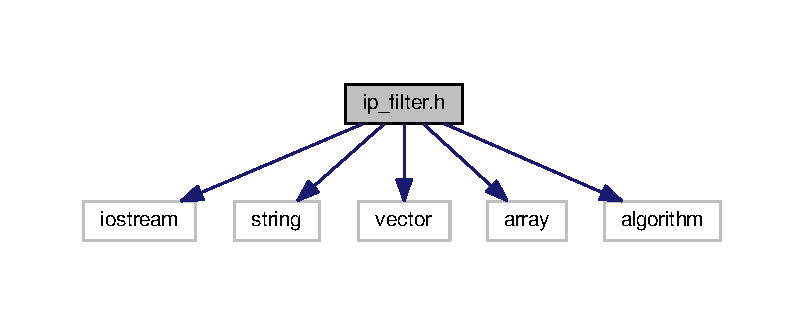
\includegraphics[width=350pt]{ip__filter_8h__incl}
\end{center}
\end{figure}
Граф файлов, в которые включается этот файл\-:
\nopagebreak
\begin{figure}[H]
\begin{center}
\leavevmode
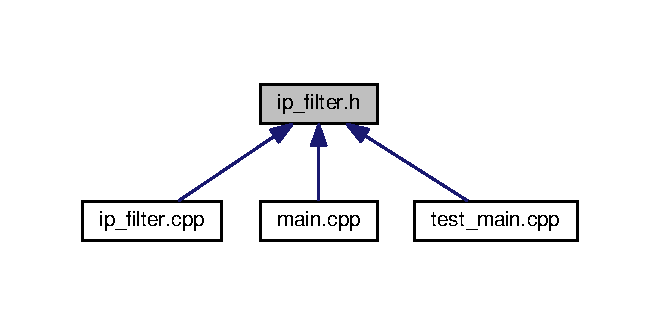
\includegraphics[width=317pt]{ip__filter_8h__dep__incl}
\end{center}
\end{figure}
\subsection*{Определения типов}
\begin{DoxyCompactItemize}
\item 
typedef std\-::array\\*
$<$ std\-::size\-\_\-t, 4 $>$ \hyperlink{ip__filter_8h_a2756a9a1f60ab937cb92e5ed91da5084}{ip\-\_\-t}
\end{DoxyCompactItemize}
\subsection*{Функции}
\begin{DoxyCompactItemize}
\item 
std\-::vector$<$ std\-::string $>$ \hyperlink{ip__filter_8h_a5d67634c85a0d90fa46ad22c5740915c}{split} (const std\-::string \&str, char d)
\item 
void \hyperlink{ip__filter_8h_a1ca671ef7008b2ca3aead135c9e72d2a}{iplist\-\_\-read} (std\-::istream \&is, std\-::vector$<$ \hyperlink{ip__filter_8h_a2756a9a1f60ab937cb92e5ed91da5084}{ip\-\_\-t} $>$ \&v)
\item 
void \hyperlink{ip__filter_8h_aeff1e0432eb5b4938e8956f988ee2bcb}{iplist\-\_\-basesort} (std\-::vector$<$ \hyperlink{ip__filter_8h_a2756a9a1f60ab937cb92e5ed91da5084}{ip\-\_\-t} $>$ \&v)
\item 
void \hyperlink{ip__filter_8h_af2cd983454a6c88e3e114902da62254b}{iplist\-\_\-print} (std\-::ostream \&os, std\-::vector$<$ \hyperlink{ip__filter_8h_a2756a9a1f60ab937cb92e5ed91da5084}{ip\-\_\-t} $>$ \&v)
\item 
{\footnotesize template$<$class Unary\-Predicate $>$ }\\void \hyperlink{ip__filter_8h_a7a2e75e6adf6d39caebb11c383b352e4}{iplist\-\_\-filter} (std\-::vector$<$ \hyperlink{ip__filter_8h_a2756a9a1f60ab937cb92e5ed91da5084}{ip\-\_\-t} $>$ \&out\-\_\-v, std\-::vector$<$ \hyperlink{ip__filter_8h_a2756a9a1f60ab937cb92e5ed91da5084}{ip\-\_\-t} $>$ \&base\-\_\-v, Unary\-Predicate p)
\end{DoxyCompactItemize}


\subsection{Типы}
\hypertarget{ip__filter_8h_a2756a9a1f60ab937cb92e5ed91da5084}{\index{ip\-\_\-filter.\-h@{ip\-\_\-filter.\-h}!ip\-\_\-t@{ip\-\_\-t}}
\index{ip\-\_\-t@{ip\-\_\-t}!ip_filter.h@{ip\-\_\-filter.\-h}}
\subsubsection[{ip\-\_\-t}]{\setlength{\rightskip}{0pt plus 5cm}typedef std\-::array$<$std\-::size\-\_\-t, 4$>$ {\bf ip\-\_\-t}}}\label{ip__filter_8h_a2756a9a1f60ab937cb92e5ed91da5084}


\subsection{Функции}
\hypertarget{ip__filter_8h_aeff1e0432eb5b4938e8956f988ee2bcb}{\index{ip\-\_\-filter.\-h@{ip\-\_\-filter.\-h}!iplist\-\_\-basesort@{iplist\-\_\-basesort}}
\index{iplist\-\_\-basesort@{iplist\-\_\-basesort}!ip_filter.h@{ip\-\_\-filter.\-h}}
\subsubsection[{iplist\-\_\-basesort}]{\setlength{\rightskip}{0pt plus 5cm}void iplist\-\_\-basesort (
\begin{DoxyParamCaption}
\item[{std\-::vector$<$ {\bf ip\-\_\-t} $>$ \&}]{v}
\end{DoxyParamCaption}
)}}\label{ip__filter_8h_aeff1e0432eb5b4938e8956f988ee2bcb}
\hypertarget{ip__filter_8h_a7a2e75e6adf6d39caebb11c383b352e4}{\index{ip\-\_\-filter.\-h@{ip\-\_\-filter.\-h}!iplist\-\_\-filter@{iplist\-\_\-filter}}
\index{iplist\-\_\-filter@{iplist\-\_\-filter}!ip_filter.h@{ip\-\_\-filter.\-h}}
\subsubsection[{iplist\-\_\-filter}]{\setlength{\rightskip}{0pt plus 5cm}template$<$class Unary\-Predicate $>$ void iplist\-\_\-filter (
\begin{DoxyParamCaption}
\item[{std\-::vector$<$ {\bf ip\-\_\-t} $>$ \&}]{out\-\_\-v, }
\item[{std\-::vector$<$ {\bf ip\-\_\-t} $>$ \&}]{base\-\_\-v, }
\item[{Unary\-Predicate}]{p}
\end{DoxyParamCaption}
)}}\label{ip__filter_8h_a7a2e75e6adf6d39caebb11c383b352e4}
\hypertarget{ip__filter_8h_af2cd983454a6c88e3e114902da62254b}{\index{ip\-\_\-filter.\-h@{ip\-\_\-filter.\-h}!iplist\-\_\-print@{iplist\-\_\-print}}
\index{iplist\-\_\-print@{iplist\-\_\-print}!ip_filter.h@{ip\-\_\-filter.\-h}}
\subsubsection[{iplist\-\_\-print}]{\setlength{\rightskip}{0pt plus 5cm}void iplist\-\_\-print (
\begin{DoxyParamCaption}
\item[{std\-::ostream \&}]{os, }
\item[{std\-::vector$<$ {\bf ip\-\_\-t} $>$ \&}]{v}
\end{DoxyParamCaption}
)}}\label{ip__filter_8h_af2cd983454a6c88e3e114902da62254b}
\hypertarget{ip__filter_8h_a1ca671ef7008b2ca3aead135c9e72d2a}{\index{ip\-\_\-filter.\-h@{ip\-\_\-filter.\-h}!iplist\-\_\-read@{iplist\-\_\-read}}
\index{iplist\-\_\-read@{iplist\-\_\-read}!ip_filter.h@{ip\-\_\-filter.\-h}}
\subsubsection[{iplist\-\_\-read}]{\setlength{\rightskip}{0pt plus 5cm}void iplist\-\_\-read (
\begin{DoxyParamCaption}
\item[{std\-::istream \&}]{is, }
\item[{std\-::vector$<$ {\bf ip\-\_\-t} $>$ \&}]{v}
\end{DoxyParamCaption}
)}}\label{ip__filter_8h_a1ca671ef7008b2ca3aead135c9e72d2a}
\hypertarget{ip__filter_8h_a5d67634c85a0d90fa46ad22c5740915c}{\index{ip\-\_\-filter.\-h@{ip\-\_\-filter.\-h}!split@{split}}
\index{split@{split}!ip_filter.h@{ip\-\_\-filter.\-h}}
\subsubsection[{split}]{\setlength{\rightskip}{0pt plus 5cm}std\-::vector$<$std\-::string$>$ split (
\begin{DoxyParamCaption}
\item[{const std\-::string \&}]{str, }
\item[{char}]{d}
\end{DoxyParamCaption}
)}}\label{ip__filter_8h_a5d67634c85a0d90fa46ad22c5740915c}

\hypertarget{main_8cpp}{\section{Файл main.\-cpp}
\label{main_8cpp}\index{main.\-cpp@{main.\-cpp}}
}
{\ttfamily \#include $<$iostream$>$}\\*
{\ttfamily \#include $<$string$>$}\\*
{\ttfamily \#include \char`\"{}version.\-h\char`\"{}}\\*
{\ttfamily \#include \char`\"{}ip\-\_\-filter.\-h\char`\"{}}\\*
Граф включаемых заголовочных файлов для main.\-cpp\-:
\nopagebreak
\begin{figure}[H]
\begin{center}
\leavevmode
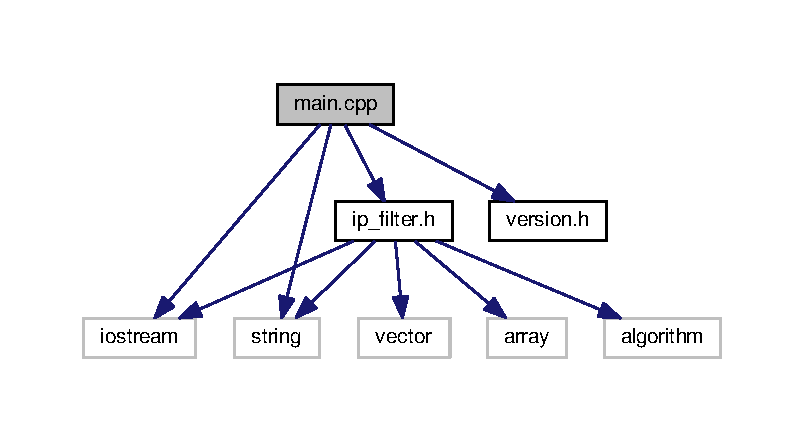
\includegraphics[width=350pt]{main_8cpp__incl}
\end{center}
\end{figure}
\subsection*{Функции}
\begin{DoxyCompactItemize}
\item 
int \hyperlink{main_8cpp_abf9e6b7e6f15df4b525a2e7705ba3089}{main} (int argc, char const $\ast$argv\mbox{[}$\,$\mbox{]})
\end{DoxyCompactItemize}


\subsection{Функции}
\hypertarget{main_8cpp_abf9e6b7e6f15df4b525a2e7705ba3089}{\index{main.\-cpp@{main.\-cpp}!main@{main}}
\index{main@{main}!main.cpp@{main.\-cpp}}
\subsubsection[{main}]{\setlength{\rightskip}{0pt plus 5cm}int main (
\begin{DoxyParamCaption}
\item[{int}]{argc, }
\item[{char const $\ast$}]{argv\mbox{[}$\,$\mbox{]}}
\end{DoxyParamCaption}
)}}\label{main_8cpp_abf9e6b7e6f15df4b525a2e7705ba3089}

\hypertarget{test__main_8cpp}{\section{Файл test\-\_\-main.\-cpp}
\label{test__main_8cpp}\index{test\-\_\-main.\-cpp@{test\-\_\-main.\-cpp}}
}
{\ttfamily \#include \char`\"{}ip\-\_\-filter.\-h\char`\"{}}\\*
{\ttfamily \#include $<$boost/test/unit\-\_\-test.\-hpp$>$}\\*
Граф включаемых заголовочных файлов для test\-\_\-main.\-cpp\-:
\nopagebreak
\begin{figure}[H]
\begin{center}
\leavevmode
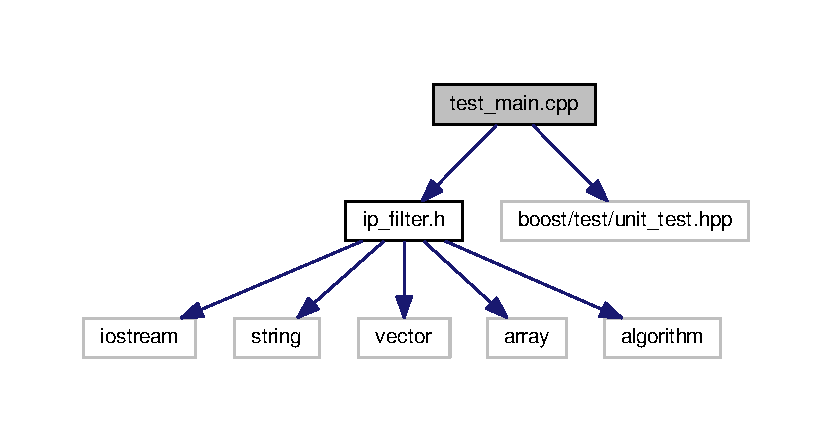
\includegraphics[width=350pt]{test__main_8cpp__incl}
\end{center}
\end{figure}
\subsection*{Макросы}
\begin{DoxyCompactItemize}
\item 
\#define \hyperlink{test__main_8cpp_a6b2a3852db8bb19ab6909bac01859985}{B\-O\-O\-S\-T\-\_\-\-T\-E\-S\-T\-\_\-\-M\-O\-D\-U\-L\-E}~test\-\_\-main
\end{DoxyCompactItemize}
\subsection*{Функции}
\begin{DoxyCompactItemize}
\item 
\hyperlink{test__main_8cpp_af28a60df7e3ccb6750024a91ff1b7604}{B\-O\-O\-S\-T\-\_\-\-A\-U\-T\-O\-\_\-\-T\-E\-S\-T\-\_\-\-C\-A\-S\-E} (test\-\_\-split)
\item 
\hyperlink{test__main_8cpp_a512f5cc34dafe0d967a9476363b4a065}{B\-O\-O\-S\-T\-\_\-\-A\-U\-T\-O\-\_\-\-T\-E\-S\-T\-\_\-\-C\-A\-S\-E} (good\-\_\-data)
\item 
\hyperlink{test__main_8cpp_ae215bc7436d5f76b4aaee6c090738624}{B\-O\-O\-S\-T\-\_\-\-A\-U\-T\-O\-\_\-\-T\-E\-S\-T\-\_\-\-C\-A\-S\-E} (empty\-\_\-data)
\item 
\hyperlink{test__main_8cpp_a946979e29fd21bc8b83efa632e5b9374}{B\-O\-O\-S\-T\-\_\-\-A\-U\-T\-O\-\_\-\-T\-E\-S\-T\-\_\-\-C\-A\-S\-E} (broken\-\_\-data)
\end{DoxyCompactItemize}


\subsection{Макросы}
\hypertarget{test__main_8cpp_a6b2a3852db8bb19ab6909bac01859985}{\index{test\-\_\-main.\-cpp@{test\-\_\-main.\-cpp}!B\-O\-O\-S\-T\-\_\-\-T\-E\-S\-T\-\_\-\-M\-O\-D\-U\-L\-E@{B\-O\-O\-S\-T\-\_\-\-T\-E\-S\-T\-\_\-\-M\-O\-D\-U\-L\-E}}
\index{B\-O\-O\-S\-T\-\_\-\-T\-E\-S\-T\-\_\-\-M\-O\-D\-U\-L\-E@{B\-O\-O\-S\-T\-\_\-\-T\-E\-S\-T\-\_\-\-M\-O\-D\-U\-L\-E}!test_main.cpp@{test\-\_\-main.\-cpp}}
\subsubsection[{B\-O\-O\-S\-T\-\_\-\-T\-E\-S\-T\-\_\-\-M\-O\-D\-U\-L\-E}]{\setlength{\rightskip}{0pt plus 5cm}\#define B\-O\-O\-S\-T\-\_\-\-T\-E\-S\-T\-\_\-\-M\-O\-D\-U\-L\-E~test\-\_\-main}}\label{test__main_8cpp_a6b2a3852db8bb19ab6909bac01859985}


\subsection{Функции}
\hypertarget{test__main_8cpp_af28a60df7e3ccb6750024a91ff1b7604}{\index{test\-\_\-main.\-cpp@{test\-\_\-main.\-cpp}!B\-O\-O\-S\-T\-\_\-\-A\-U\-T\-O\-\_\-\-T\-E\-S\-T\-\_\-\-C\-A\-S\-E@{B\-O\-O\-S\-T\-\_\-\-A\-U\-T\-O\-\_\-\-T\-E\-S\-T\-\_\-\-C\-A\-S\-E}}
\index{B\-O\-O\-S\-T\-\_\-\-A\-U\-T\-O\-\_\-\-T\-E\-S\-T\-\_\-\-C\-A\-S\-E@{B\-O\-O\-S\-T\-\_\-\-A\-U\-T\-O\-\_\-\-T\-E\-S\-T\-\_\-\-C\-A\-S\-E}!test_main.cpp@{test\-\_\-main.\-cpp}}
\subsubsection[{B\-O\-O\-S\-T\-\_\-\-A\-U\-T\-O\-\_\-\-T\-E\-S\-T\-\_\-\-C\-A\-S\-E}]{\setlength{\rightskip}{0pt plus 5cm}B\-O\-O\-S\-T\-\_\-\-A\-U\-T\-O\-\_\-\-T\-E\-S\-T\-\_\-\-C\-A\-S\-E (
\begin{DoxyParamCaption}
\item[{test\-\_\-split}]{}
\end{DoxyParamCaption}
)}}\label{test__main_8cpp_af28a60df7e3ccb6750024a91ff1b7604}
\hypertarget{test__main_8cpp_a512f5cc34dafe0d967a9476363b4a065}{\index{test\-\_\-main.\-cpp@{test\-\_\-main.\-cpp}!B\-O\-O\-S\-T\-\_\-\-A\-U\-T\-O\-\_\-\-T\-E\-S\-T\-\_\-\-C\-A\-S\-E@{B\-O\-O\-S\-T\-\_\-\-A\-U\-T\-O\-\_\-\-T\-E\-S\-T\-\_\-\-C\-A\-S\-E}}
\index{B\-O\-O\-S\-T\-\_\-\-A\-U\-T\-O\-\_\-\-T\-E\-S\-T\-\_\-\-C\-A\-S\-E@{B\-O\-O\-S\-T\-\_\-\-A\-U\-T\-O\-\_\-\-T\-E\-S\-T\-\_\-\-C\-A\-S\-E}!test_main.cpp@{test\-\_\-main.\-cpp}}
\subsubsection[{B\-O\-O\-S\-T\-\_\-\-A\-U\-T\-O\-\_\-\-T\-E\-S\-T\-\_\-\-C\-A\-S\-E}]{\setlength{\rightskip}{0pt plus 5cm}B\-O\-O\-S\-T\-\_\-\-A\-U\-T\-O\-\_\-\-T\-E\-S\-T\-\_\-\-C\-A\-S\-E (
\begin{DoxyParamCaption}
\item[{good\-\_\-data}]{}
\end{DoxyParamCaption}
)}}\label{test__main_8cpp_a512f5cc34dafe0d967a9476363b4a065}
\hypertarget{test__main_8cpp_ae215bc7436d5f76b4aaee6c090738624}{\index{test\-\_\-main.\-cpp@{test\-\_\-main.\-cpp}!B\-O\-O\-S\-T\-\_\-\-A\-U\-T\-O\-\_\-\-T\-E\-S\-T\-\_\-\-C\-A\-S\-E@{B\-O\-O\-S\-T\-\_\-\-A\-U\-T\-O\-\_\-\-T\-E\-S\-T\-\_\-\-C\-A\-S\-E}}
\index{B\-O\-O\-S\-T\-\_\-\-A\-U\-T\-O\-\_\-\-T\-E\-S\-T\-\_\-\-C\-A\-S\-E@{B\-O\-O\-S\-T\-\_\-\-A\-U\-T\-O\-\_\-\-T\-E\-S\-T\-\_\-\-C\-A\-S\-E}!test_main.cpp@{test\-\_\-main.\-cpp}}
\subsubsection[{B\-O\-O\-S\-T\-\_\-\-A\-U\-T\-O\-\_\-\-T\-E\-S\-T\-\_\-\-C\-A\-S\-E}]{\setlength{\rightskip}{0pt plus 5cm}B\-O\-O\-S\-T\-\_\-\-A\-U\-T\-O\-\_\-\-T\-E\-S\-T\-\_\-\-C\-A\-S\-E (
\begin{DoxyParamCaption}
\item[{empty\-\_\-data}]{}
\end{DoxyParamCaption}
)}}\label{test__main_8cpp_ae215bc7436d5f76b4aaee6c090738624}
\hypertarget{test__main_8cpp_a946979e29fd21bc8b83efa632e5b9374}{\index{test\-\_\-main.\-cpp@{test\-\_\-main.\-cpp}!B\-O\-O\-S\-T\-\_\-\-A\-U\-T\-O\-\_\-\-T\-E\-S\-T\-\_\-\-C\-A\-S\-E@{B\-O\-O\-S\-T\-\_\-\-A\-U\-T\-O\-\_\-\-T\-E\-S\-T\-\_\-\-C\-A\-S\-E}}
\index{B\-O\-O\-S\-T\-\_\-\-A\-U\-T\-O\-\_\-\-T\-E\-S\-T\-\_\-\-C\-A\-S\-E@{B\-O\-O\-S\-T\-\_\-\-A\-U\-T\-O\-\_\-\-T\-E\-S\-T\-\_\-\-C\-A\-S\-E}!test_main.cpp@{test\-\_\-main.\-cpp}}
\subsubsection[{B\-O\-O\-S\-T\-\_\-\-A\-U\-T\-O\-\_\-\-T\-E\-S\-T\-\_\-\-C\-A\-S\-E}]{\setlength{\rightskip}{0pt plus 5cm}B\-O\-O\-S\-T\-\_\-\-A\-U\-T\-O\-\_\-\-T\-E\-S\-T\-\_\-\-C\-A\-S\-E (
\begin{DoxyParamCaption}
\item[{broken\-\_\-data}]{}
\end{DoxyParamCaption}
)}}\label{test__main_8cpp_a946979e29fd21bc8b83efa632e5b9374}

\hypertarget{version_8h}{\section{Файл version.\-h}
\label{version_8h}\index{version.\-h@{version.\-h}}
}
Граф файлов, в которые включается этот файл\-:
\nopagebreak
\begin{figure}[H]
\begin{center}
\leavevmode
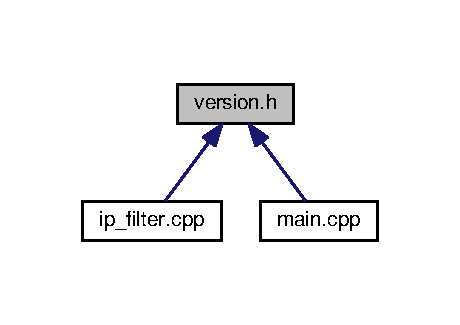
\includegraphics[width=221pt]{version_8h__dep__incl}
\end{center}
\end{figure}
\subsection*{Макросы}
\begin{DoxyCompactItemize}
\item 
\#define \hyperlink{version_8h_abecd2198575b690d25a741857f8390d1}{P\-R\-O\-J\-E\-C\-T\-\_\-\-V\-E\-R\-S\-I\-O\-N\-\_\-\-M\-A\-J\-O\-R}~0
\item 
\#define \hyperlink{version_8h_a43e23009192a3e216fefec17750d8673}{P\-R\-O\-J\-E\-C\-T\-\_\-\-V\-E\-R\-S\-I\-O\-N\-\_\-\-M\-I\-N\-O\-R}~0
\item 
\#define \hyperlink{version_8h_a4a5fc96a4bdd7d68ed99ccce9ca2e77e}{P\-R\-O\-J\-E\-C\-T\-\_\-\-V\-E\-R\-S\-I\-O\-N\-\_\-\-P\-A\-T\-C\-H}~4
\end{DoxyCompactItemize}


\subsection{Макросы}
\hypertarget{version_8h_abecd2198575b690d25a741857f8390d1}{\index{version.\-h@{version.\-h}!P\-R\-O\-J\-E\-C\-T\-\_\-\-V\-E\-R\-S\-I\-O\-N\-\_\-\-M\-A\-J\-O\-R@{P\-R\-O\-J\-E\-C\-T\-\_\-\-V\-E\-R\-S\-I\-O\-N\-\_\-\-M\-A\-J\-O\-R}}
\index{P\-R\-O\-J\-E\-C\-T\-\_\-\-V\-E\-R\-S\-I\-O\-N\-\_\-\-M\-A\-J\-O\-R@{P\-R\-O\-J\-E\-C\-T\-\_\-\-V\-E\-R\-S\-I\-O\-N\-\_\-\-M\-A\-J\-O\-R}!version.h@{version.\-h}}
\subsubsection[{P\-R\-O\-J\-E\-C\-T\-\_\-\-V\-E\-R\-S\-I\-O\-N\-\_\-\-M\-A\-J\-O\-R}]{\setlength{\rightskip}{0pt plus 5cm}\#define P\-R\-O\-J\-E\-C\-T\-\_\-\-V\-E\-R\-S\-I\-O\-N\-\_\-\-M\-A\-J\-O\-R~0}}\label{version_8h_abecd2198575b690d25a741857f8390d1}
\hypertarget{version_8h_a43e23009192a3e216fefec17750d8673}{\index{version.\-h@{version.\-h}!P\-R\-O\-J\-E\-C\-T\-\_\-\-V\-E\-R\-S\-I\-O\-N\-\_\-\-M\-I\-N\-O\-R@{P\-R\-O\-J\-E\-C\-T\-\_\-\-V\-E\-R\-S\-I\-O\-N\-\_\-\-M\-I\-N\-O\-R}}
\index{P\-R\-O\-J\-E\-C\-T\-\_\-\-V\-E\-R\-S\-I\-O\-N\-\_\-\-M\-I\-N\-O\-R@{P\-R\-O\-J\-E\-C\-T\-\_\-\-V\-E\-R\-S\-I\-O\-N\-\_\-\-M\-I\-N\-O\-R}!version.h@{version.\-h}}
\subsubsection[{P\-R\-O\-J\-E\-C\-T\-\_\-\-V\-E\-R\-S\-I\-O\-N\-\_\-\-M\-I\-N\-O\-R}]{\setlength{\rightskip}{0pt plus 5cm}\#define P\-R\-O\-J\-E\-C\-T\-\_\-\-V\-E\-R\-S\-I\-O\-N\-\_\-\-M\-I\-N\-O\-R~0}}\label{version_8h_a43e23009192a3e216fefec17750d8673}
\hypertarget{version_8h_a4a5fc96a4bdd7d68ed99ccce9ca2e77e}{\index{version.\-h@{version.\-h}!P\-R\-O\-J\-E\-C\-T\-\_\-\-V\-E\-R\-S\-I\-O\-N\-\_\-\-P\-A\-T\-C\-H@{P\-R\-O\-J\-E\-C\-T\-\_\-\-V\-E\-R\-S\-I\-O\-N\-\_\-\-P\-A\-T\-C\-H}}
\index{P\-R\-O\-J\-E\-C\-T\-\_\-\-V\-E\-R\-S\-I\-O\-N\-\_\-\-P\-A\-T\-C\-H@{P\-R\-O\-J\-E\-C\-T\-\_\-\-V\-E\-R\-S\-I\-O\-N\-\_\-\-P\-A\-T\-C\-H}!version.h@{version.\-h}}
\subsubsection[{P\-R\-O\-J\-E\-C\-T\-\_\-\-V\-E\-R\-S\-I\-O\-N\-\_\-\-P\-A\-T\-C\-H}]{\setlength{\rightskip}{0pt plus 5cm}\#define P\-R\-O\-J\-E\-C\-T\-\_\-\-V\-E\-R\-S\-I\-O\-N\-\_\-\-P\-A\-T\-C\-H~4}}\label{version_8h_a4a5fc96a4bdd7d68ed99ccce9ca2e77e}

%--- End generated contents ---

% Index
\newpage
\phantomsection
\addcontentsline{toc}{chapter}{Алфавитный указатель}
\printindex

\end{document}
